%%%% 3D Skewness Example %%%%%%

\subsection{Dependence on Dimension}\label{ex:3dmap}
To further illustrate that relationship between skewness and accuracy holds as we move towards higher dimensions, we extend the numerical investigation to a three--dimensional parameter space.
Generally, we have fewer QoI than number of uncertain model parameters, so we assume that the potential QoI maps are defined by the $2\times 3$ matrices
\begin{equation}\label{eq:qmap3}
\qspace_S := \left \lbrace \qoi^{(s)} =  \mat{ccc}{1 & 0 & 0\\ \sqrt{s^2 - 1}& 1 & 0} \right \rbrace_{s\in S}.
\end{equation}
Here, as in the previous example, the index $s$ indicates the magnitude of skewness.
Furthermore, the results of Example~\ref{ex:rotation} justify the restriction of the maps to this form since any linear map of skewness $s$ is simply a rotation of maps of this form.

%Now, the generalized contours for inverses of maps from $\RR^3 \to \RR^2$ will be isomorphic to 2\--dimensional contour events in that the inverse sets will be columns in 3\-space orthogonal to the aforemntioned plane.
%
%IMAGE DEMONSTRATING THIS WOULD HELP.
%We define
%
%which is just the map from \eqref{eq:qmap2} appended with zeros in the third column.
%We make this choice solely for convience and are justified in doing so owing to Proposition~\ref{prop:rot_invariance} and the fact of generalized contours of maps from $\RR^3 \to \RR^2$ being parallel columns.
%The rotational invariance naturally extends to the third dimension.

%We note that $\bar{N}$ is much higher since we kept the convention of 200 grid cells per dimension in our reference.
%However, we kept the same number of random samples $N$, so we should expect higher errors due to the overresolved regular grid.
%Fortunately, we find that the results still generalize.
%We present the case where $M=1$:

\begin{figure}[h]
\begin{minipage}{.5\textwidth}
\begin{table}[H]
\begin{tabular}{ c | c | c | c }
\nsamps & $\qoiA$ & $\qoiB$ & $\qoiC$\\ \hline \hline
$200$ & $2.98E-01$ & $4.18E-01$ & $5.60E-01$\\ \hline

$400$ & $2.27E-01$ & $3.27E-01$ & $4.69E-01$\\ \hline

$800$ & $1.81E-01$ & $2.70E-01$ & $3.97E-01$\\ \hline

$1600$ & $1.46E-01$ & $2.15E-01$ & $3.09E-01$\\ \hline

$3200$ & $1.15E-01$ & $1.72E-01$ & $2.44E-01$\\ \hline

$6400$ & $9.09E-02$ & $1.39E-01$ & $1.95E-01$\\ \hline
\end{tabular}
\end{table}
\end{minipage}
\begin{minipage}{.45\textwidth}
		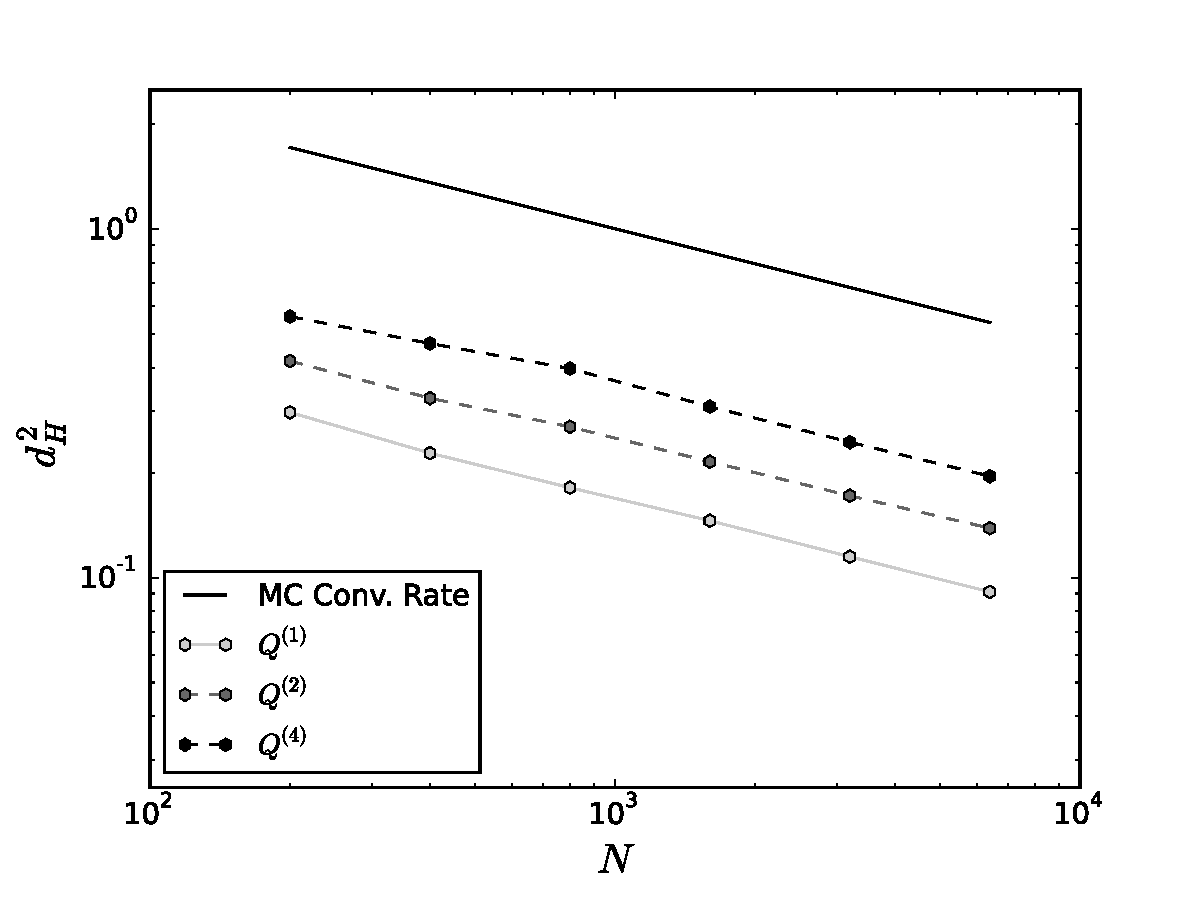
\includegraphics[width=\linewidth]{./images/Plot-reg_BigN_8000000_reg_M_1_rand_I_100000}
\end{minipage}
\caption{The results of $d^2_H(\PP_{\pspace, \ndiscs, \nsamps}, \PP_{\pspace, \ndiscs, \bar{\nsamps}})$ for $\ndiscs = 1, \bar{\nsamps} = 8,000,000$, with $a, b, c = 1, 2, 4$.}
\label{fig:M1_3d}
\end{figure}
\FloatBarrier
In Figure~\ref{fig:M1_3d}, it appears that the effect of skewness is even more pronounced in higher dimensions, and that the number of samples required to achieve similar levels of accuracy between two maps with a ratio of skewness 2 is now quadrupled.
The analysis of \cite{BGE+15} suggested a dependence of accuracy related to the skewness raised to a power related to the dimension of the data space.
